\documentclass{standalone}
\usepackage[T1]{fontenc}
\usepackage[latin2]{inputenc}
\usepackage[english]{babel}
\usepackage{tikz}
\usetikzlibrary{calc,through,backgrounds,positioning,fit}
\usetikzlibrary{shapes,arrows,shadows}
 
\begin{document}
 
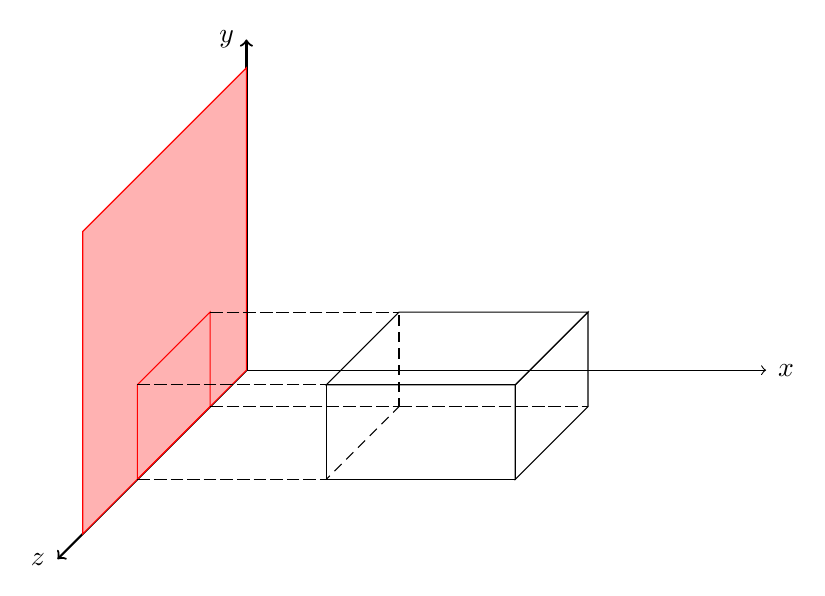
\begin{tikzpicture}[scale=1.2,inner sep=0.4mm]

\draw[thin] [->] (0,0) -- (5.5,0)node[right=3pt] {
$x$};
\draw[thick] [->] (0,0) -- (0,3.5)node[left=3pt] {$y$};
\draw[thick] [->] (0,0) -- (-2,-2)node[left=3pt] {$z$};
\filldraw[draw=red,fill=red!30!white] (0,0,0) -- (0,0,4.5)-- (0,3.2,4.5) --(0,3.2,0) --cycle;
\draw[red] (0,0,1) -- (0,1,1)-- (0,1,3) --(0,0,3) --cycle;

\draw[dashed] (0,0,1) -- (2,0,1) --cycle;
\draw[dashed] (0,0,3) -- (2,0,3) --cycle;
\draw[dashed] (0,1,1) -- (2,1,1) --cycle;
\draw[dashed] (0,1,3) -- (2,1,3) --cycle;

\draw[dashed] (2,0,1) -- (2,1,1) --cycle;
\draw[] (4,0,1) -- (4,0,3)-- (4,1,3) --(4,1,1) --cycle;

\draw[dashed] (2,0,1) -- (2,0,3) --cycle;
\draw[dashed] (2,0,1) --(4,0,1) --cycle;


\draw[] (2,1,1) -- (2,1,3)-- (4,1,3) --(4,1,1) --cycle;
\draw[] (2,0,3) -- (2,1,3)-- (4,1,3) --(4,0,3) --cycle;





\end{tikzpicture}
 
\end{document}